\usepackage{etoolbox}

% % beamer background template
% \setbeamercolor{background canvas}{bg=yellow!20}
% note that the term "standout" is special

\defbeamertemplate{background canvas}{calmlush}{%
  \color{yellow!40}\vrule width\paperwidth height\paperheight% added calmlush color
}

% \defbeamertemplate{background canvas}{standout}{%
%   \parbox[c][\paperheight][c]{\paperwidth}{\centering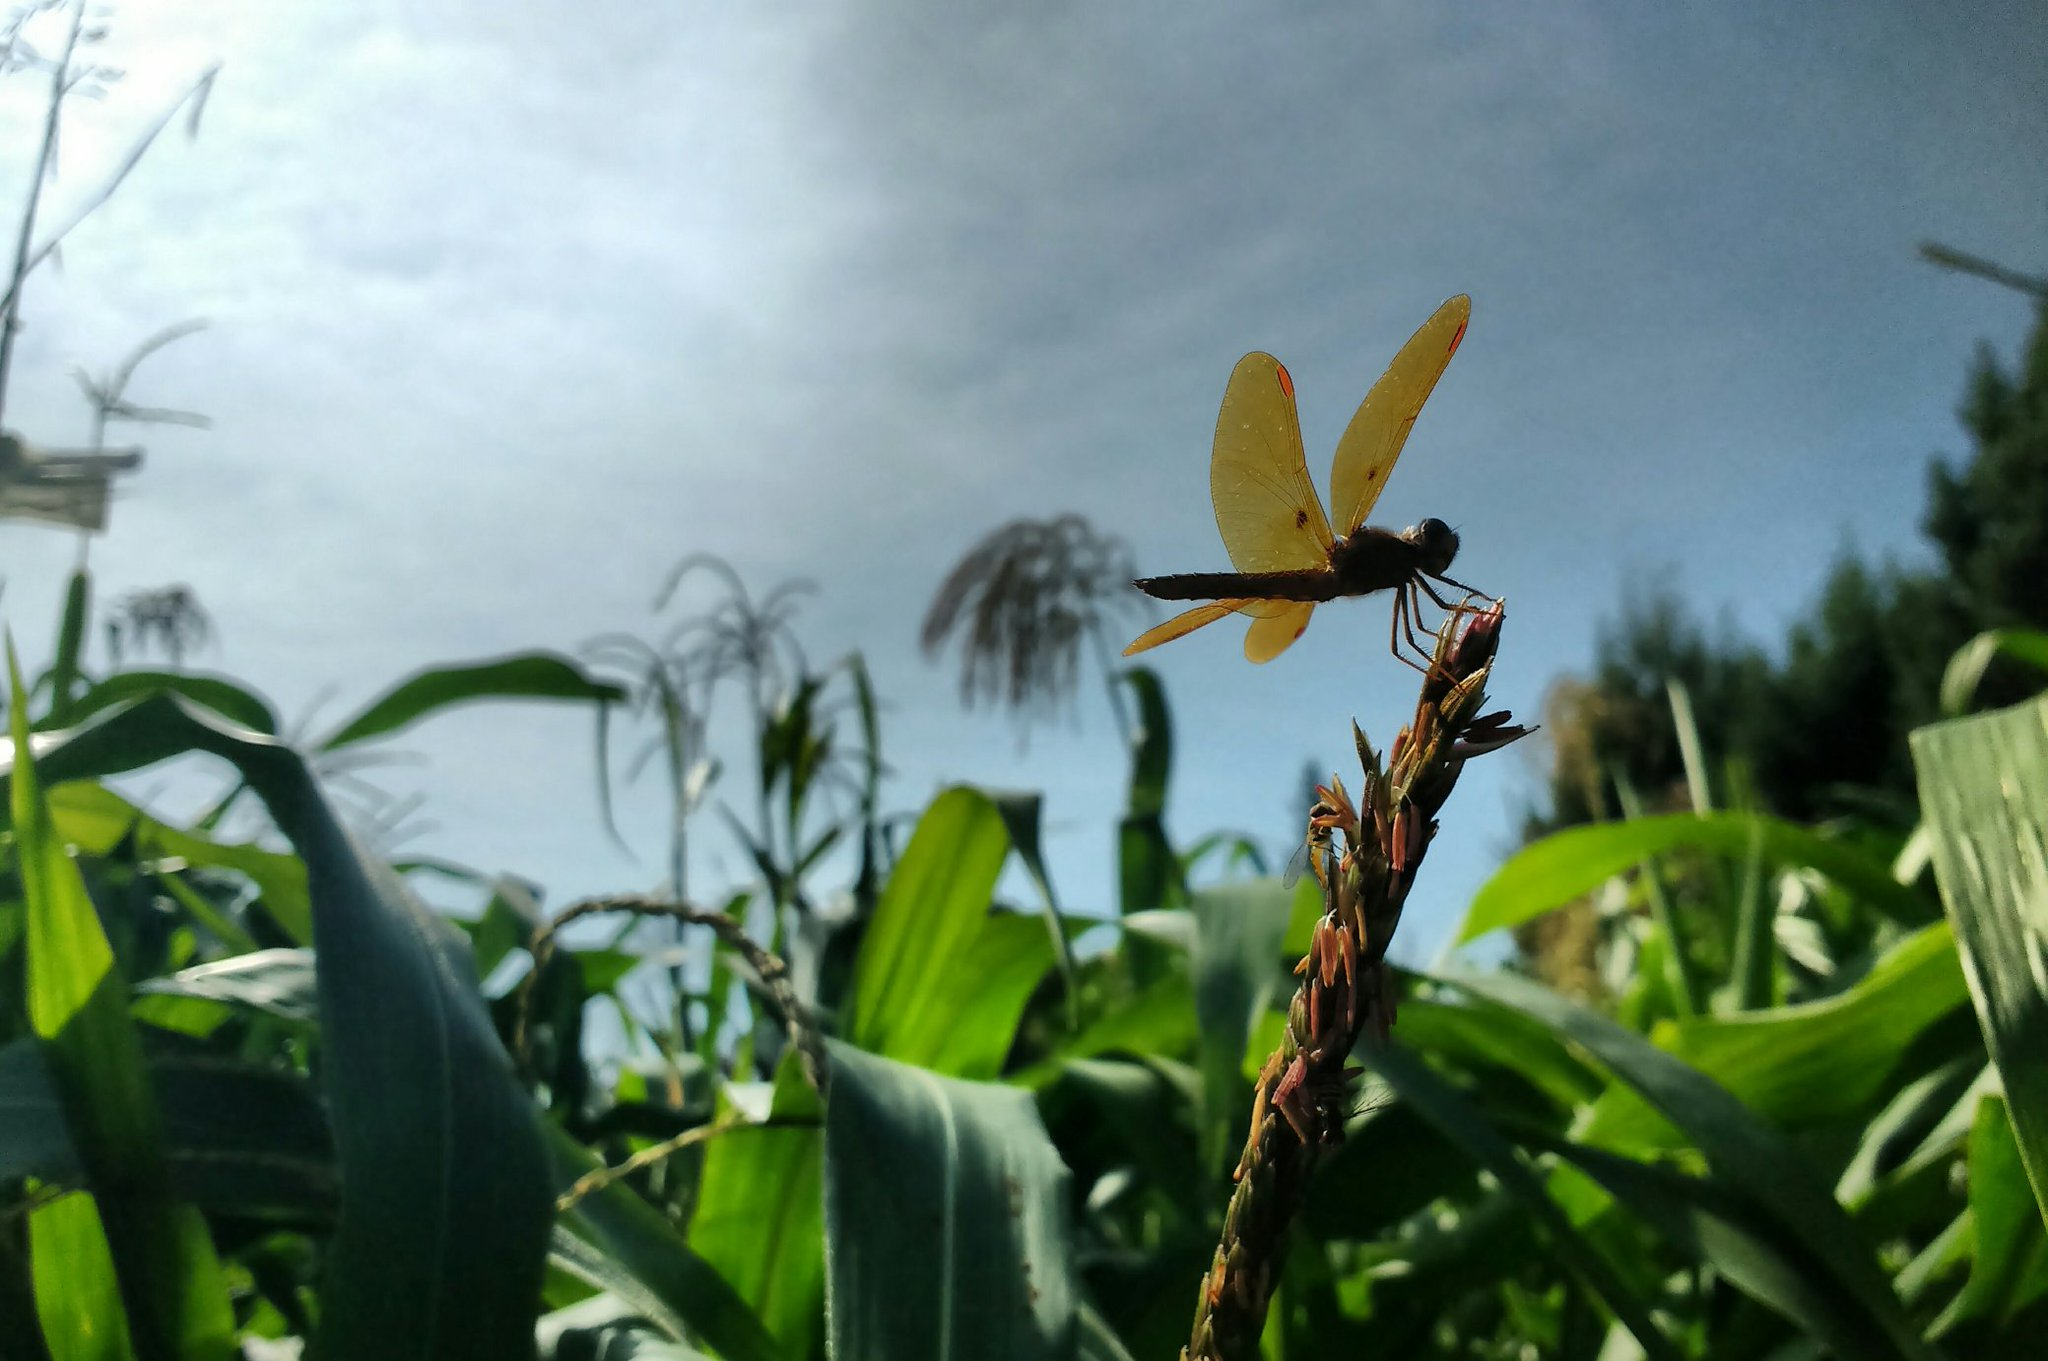
\includegraphics[width=1.2\paperwidth,height=1.2\paperheight,keepaspectratio]{images/Teosinte_dragonfly.jpg}}
% }

\defbeamertemplate{background canvas}{standout}{%
  \parbox[c][\paperheight][c]{\paperwidth}{\centering\tikz\node[opacity=0.5]{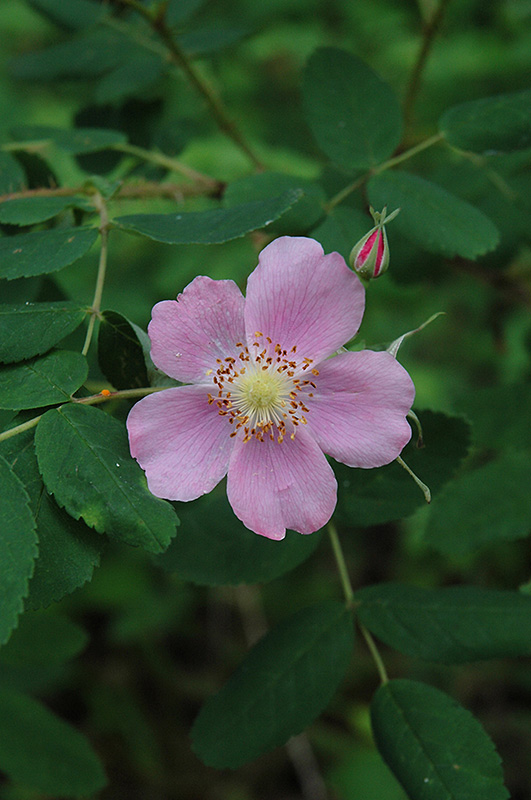
\includegraphics[width=1.2\paperwidth,height=1.2\paperheight,keepaspectratio]{images/rose_prickly_or_common2.jpg}};}
}

\BeforeBeginEnvironment{frame}{%
  \setbeamertemplate{background canvas}[calmlush]%
}

\makeatletter
\define@key{beamerframe}{standout}[true]{%
  \setbeamertemplate{background canvas}[standout]%
}
\makeatother



% % change background
% \defbeamertemplate{background canvas}{standout}{%
%   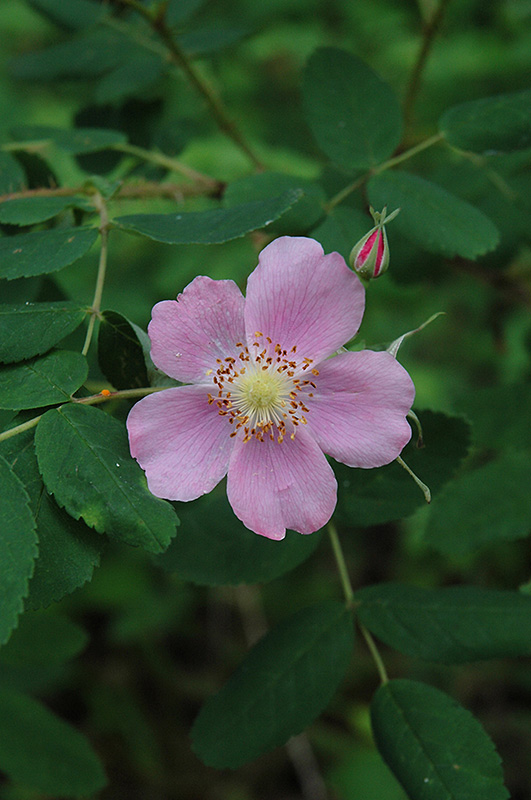
\includegraphics[width=\paperwidth,height=\paperheight,keepaspectratio]{images/rose_prickly_or_common2.jpg}
% }
% 
% \defbeamertemplate{background canvas}{standout}{%
%   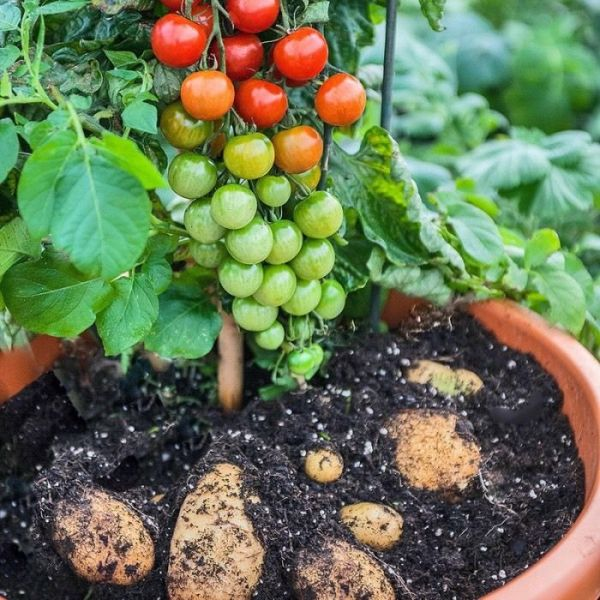
\includegraphics[width=\paperwidth,height=\paperheight,keepaspectratio]{images/pomato_hybrid_graft.jpg}
% }